\paragraph{Ausschalten von DHCP}
\begin{figure}[!htb]
    \centering
    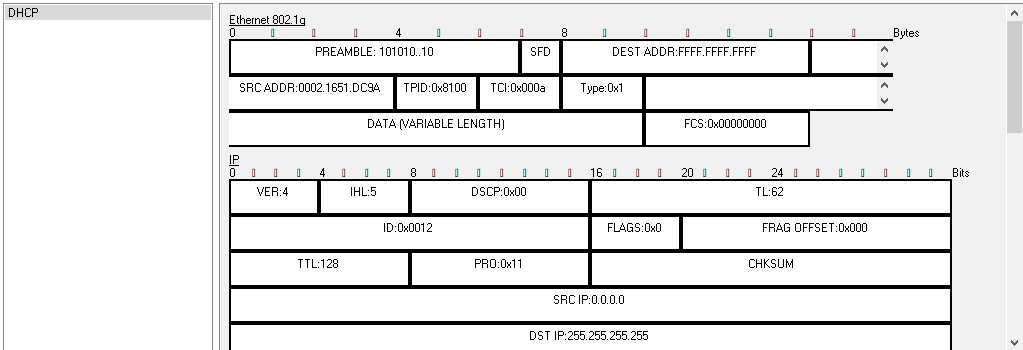
\includegraphics[width=\textwidth,height=.85\textwidth,keepaspectratio]{./img/dhcp_aus.png}
    \caption{Sniffer}
\end{figure}
\noindent
Sobald beim Endsystem auf static geschaltet wurde, hat das Endsystem ein Broadcast gemacht um die eigene Adresse zu erhalten, welche aber nicht mehr von DHCP Server kommt. Bei einem DHCP wird immer mit 0.0.0.0 als Src und 255.255.255.255 als Dest nach einer Adresse angefragt.
\paragraph{Einschalten von DHCP}
1.DHCP Discover: Der Client fragt nach einer Adresse in dem er einen Broadcast mit 0.0.0.0 als Src und 255.255.255.255 als Dest macht.\\
2.DHCP Offer: Als Antwort bekommt er dann eine Adresse vom Server "geoffert".\\
3.DHCP Request: Wenn der Client die Addresse bekommt, schickt er dem Server ein Request um diese Adresse für ihn zu übernehmen/allokieren.\\
4.DHCP ACK: Der Server sendet die Infos, die der Client braucht um konfiguriert zu werden.
\pagebreak

\subsubsection{Frage 3}
\paragraph{Frage}
Frage 3: Warum scheinen im Trace des Sniffers alle Nachrichten doppelt auf?
\paragraph{Antwort}
Die Nachrichten tauchen nur einmal auf.
\begin{figure}[!htb]
    \centering
    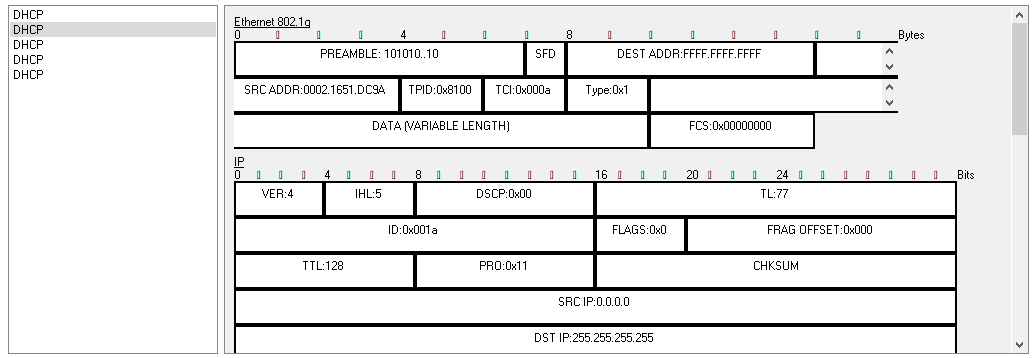
\includegraphics[width=\textwidth,height=.85\textwidth,keepaspectratio]{./img/dhcp_ein.png}
    \caption{Sniffer}
\end{figure}